% Revisão consolidada: 25/11/2026. Não antecipa resultados finais.
\chapter{Desenvolvimento mecânico}
\section{Estrutura e princípio de dispensação}
O conjunto organiza a central, os intermediários e os submódulos removíveis. Em vez de compartimentos abastecidos por horário, cada reservatório é associado a um medicamento, e o disco busca separar a quantidade requerida. O material descreve reservatório, disco de cavidades, placa de apoio, acoplamento, trajeto de queda e recipiente coletor. Isso caracteriza a concepção; desempenho e limites por comprimido dependem de ensaio. \cite{DC_PREREL,DC_COMPILADO}
\section{Disco, inclinação e sequência funcional}
Adota-se 35\ensuremath{^{\circ}} como inclinação de projeto, conforme a decisão da autora e o pré-relatório. Não se trata de medida do conjunto impresso. O disco documentado tem cinco cavidades e é acionado pelo motor de passo. Capturar, transportar, liberar e reler a cavidade são etapas distintas. Não se assume que um avanço de uma cavidade correspondeu a uma unidade liberada. \cite{DC_PREREL,DC_COMPILADO}
\pendencia{MEC01}{Inserir CAD e desenho técnico finais, revisão, cotas e relação das peças fabricadas com o modelo. A inclinação adotada é 35\ensuremath{^{\circ}}; fornecer a evidência de fabricação e a medição do conjunto montado.}
\section{Dimensões recuperadas do modelo V75}
O compilado registra medidas extraídas do modelo digital V75. Elas ajudam a identificar peças e pontos críticos, mas não são medições físicas nem prova de correspondência com a versão escolhida. O V75 indica inclinação de 30\ensuremath{^{\circ}}, divergente dos 35\ensuremath{^{\circ}} adotados nesta revisão. Portanto, esses valores permanecem identificados como referência geométrica histórica. \cite{DC_COMPILADO}

{\small\setlength{\tabcolsep}{3pt}\begin{longtable}{p{0.25\textwidth}p{0.32\textwidth}p{0.31\textwidth}}\caption{Medidas documentais do V75, não verificadas na peça fabricada}\label{tab:07-1}\\
\hline
\textbf{Referência no V75} & \textbf{Valor documental} & \textbf{Limitação}\\\hline
\endfirsthead\hline
\textbf{Referência no V75} & \textbf{Valor documental} & \textbf{Limitação}\\\hline
\endhead
Disco & 57,3 mm de diâmetro; placa de 6,0 mm & Modelo digital; confirmar peça.\\\hline
Cavidades & Cinco furos de 11,0 mm; círculo de 39,6 mm & Confirmar geometria e medicamento compatível.\\\hline
Folga disco--reservatório & 0,72 mm na direção do eixo & Não medida após impressão.\\\hline
Canal vertical central & 30 mm & Não utilizar 60 mm de outro conceito.\\\hline
Copo coletor & 38,0 mm externos; parede aproximada de 1,5 mm; altura 34 mm & Confirmar se é o coletor instalado.\\\hline
Inclinação da referência & 30\ensuremath{^{\circ}} no V75; 35\ensuremath{^{\circ}} adotados para o projeto & Revisão CAD e medida física pendentes.\\\hline
\end{longtable}}{\small\noindent Fonte: Compilado da equipe, medidas recuperadas do modelo V75.\par}


\pendencia{MEC03}{Conferir as dimensões da peça fabricada com instrumento, revisão e incerteza apropriados. Medir disco, cavidades, folgas, aberturas, oscilação e trajeto até o coletor. Não converter cotas do V75 em valores medidos do protótipo.}
\section{Modelos apresentados no artigo}
As figuras permitem identificar o conceito mecânico e as partes do dosador no artigo. Não possuem, por si, identificação suficiente de revisão, material ou parâmetros de impressão; tampouco comprovam a inclinação da peça final. \cite{DC_ARTIGO}
\begin{figure}[htbp]\centering
\caption{Representação do reservatório e do disco no artigo, utilizada como referência conceitual.}
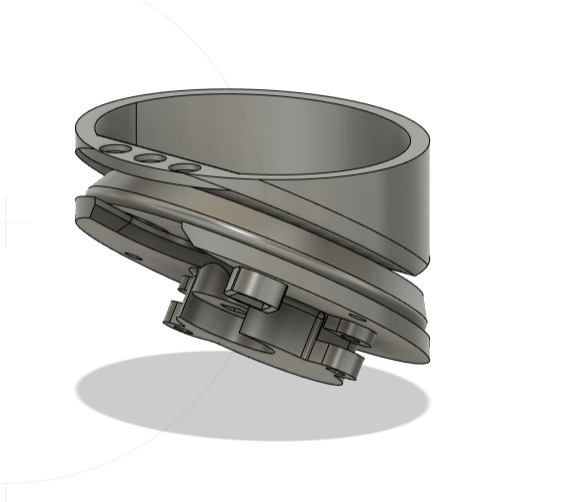
\includegraphics[width=0.82\textwidth,height=0.55\textheight,keepaspectratio]{Figuras/Artigo/cad_funil_artigo.jpeg}
\fonte{Artigo e Anexo A, versão 2, material da equipe \cite{DC_ARTIGO}.}\end{figure}
\begin{figure}[htbp]\centering
\caption{Vista inferior do componente dosador apresentada no artigo.}
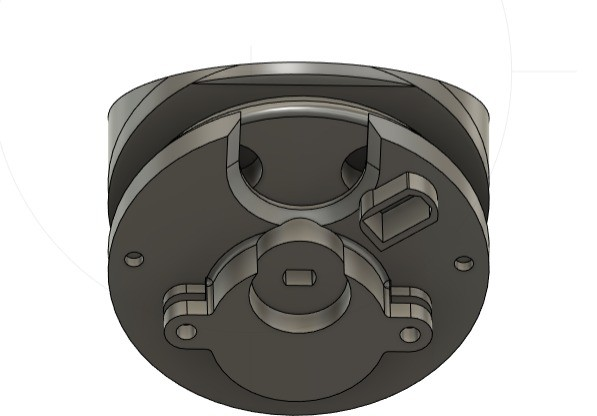
\includegraphics[width=0.82\textwidth,height=0.55\textheight,keepaspectratio]{Figuras/Artigo/cad_modulo_artigo.jpeg}
\fonte{Artigo e Anexo A, versão 2, material da equipe \cite{DC_ARTIGO}.}\end{figure}
A representação do conjunto completo no artigo é apresentada a seguir. Trata-se de modelo CAD, não de fotografia do protótipo montado nem de comprovação de ensaio. \cite{DC_ARTIGO}
\begin{figure}[htbp]\centering
\caption{Representação CAD do conjunto completo apresentada no artigo.}
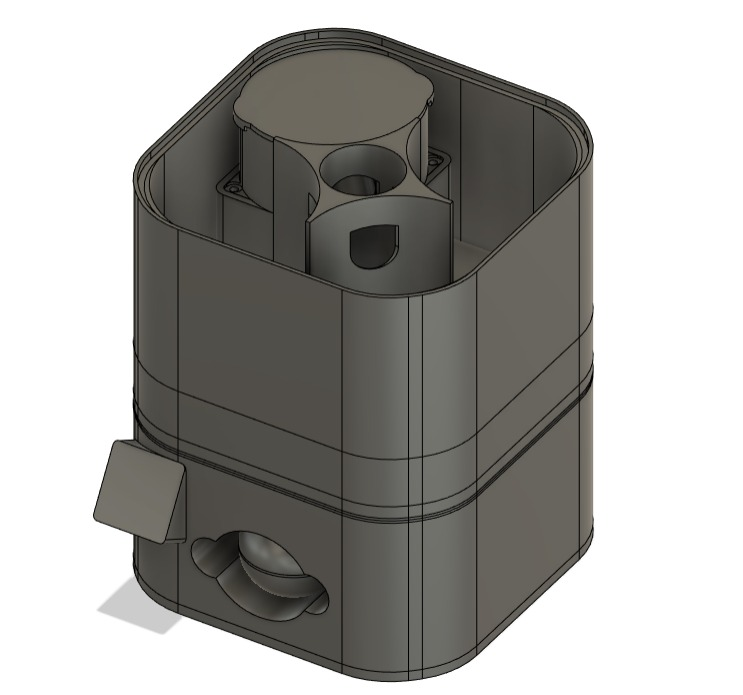
\includegraphics[width=0.65\textwidth,height=0.48\textheight,keepaspectratio]{Figuras/Artigo/conjunto_completo_artigo.jpeg}
\fonte{Artigo e Anexo A, versão 2, material da equipe \cite{DC_ARTIGO}.}
\end{figure}

\section{Materiais, impressão e fixação}
As listas fornecidas preveem PLA branco, parafusos M3 e ímãs. Material comprado não equivale a material usado em cada peça. O compilado descreve alojamentos e folgas no V75 e recomenda registrar parâmetros por componente. Não foi fornecido nesta rodada o material complementar prometido com o inventário final instalado. \cite{DC_LISTA,DC_PROPOSTA,DC_COMPILADO}
\pendencia{MEC04}{Inserir a ficha de fabricação por peça: material/marca/lote, impressora, fatiador, revisão, bico, temperaturas, camada, perímetros, preenchimento, orientação, suportes, tempo e massa. A lista de compra já foi recebida; falta a fabricação efetiva.}
\pendencia{MEC05}{Completar a lista técnica instalada: parafusos por posição, ímãs e polaridade, acoplamentos, pogo, retenção, ajustes e eventual uso de adesivo. Incorporar o material complementar a ser fornecido pela autora.}
\section{Montagem, manutenção e limpeza}
A remoção do submódulo é um requisito de projeto, mas demanda verificar retenção, alinhamento e continuidade durante ciclos de encaixe. O funcionamento com medicamentos exige também conhecer o acabamento das superfícies, o procedimento de limpeza e a possibilidade de retenção de resíduos. Não há base para declarar adequação sanitária ou durabilidade sem esses registros. \cite{DC_COMPILADO}
\pendencia{MEC06-FOTO1}{INSERIR FOTO: vista geral do protótipo físico final, identificando revisão, módulos presentes e data. A figura CAD do artigo não substitui a fotografia.}
\pendencia{MEC06-FOTO2}{INSERIR FOTOS: disco, cavidades, reservatório, placa de apoio, saída, coletor, fixação do motor e contatos. Incluir escala e legenda, sem dados pessoais.}
\section{Verificações mecânicas pendentes}
\pendencia{MEC07}{Registrar massas, inclinação medida, atrito/ângulo de deslizamento, retenção desenergizada, folgas após impressão, desgaste e ciclos de encaixe. Para cada tipo de comprimido de teste, registrar captura simples/dupla, retenção, travamento, tentativas e falhas com denominador. Não há resultados finais fornecidos.}
